\chapter{Introduction to Deep Learning and Neural Architectures}
Let us now take a step back and think about the initial developments of artificial intelligence. Since their early days, AI-powered systems have been able to tackle and solve problems that had proven to be very difficult for humans, such as those that could be described by a list of formal and mathematical rules. The true challenge to artificial intelligence proved in fact to be solving tasks that are easy for people to perform, but hard for people to describe formally: problems that we solve intuitively, that feel automatic, like recognizing spoken words or faces in images. Several attempts were made to hard-code knowledge about the world in formal languages, but they were never able to achieve major successes.

Much of our knowledge is in fact based on \textbf{unstructured} inputs: computers then need to be able to capture this same knowledge and extract patterns from raw data, in order to behave in an intelligent way. \textbf{Machine learning} techniques can help in accomplishing this, enabling classification, clustering and rule discovery when given in input the right set of \textbf{features}. For many tasks, however, it is difficult to know which features should be extracted (like when recognizing objects in a photo, emotions from speech, etc.) and how information is structured and ``represented''. One solution to this problem is to use machine learning to discover not only the mapping from representation to output, but also the representation itself, with an approach known as \textbf{representation learning}. Learned representations often result in much better performance than the one that can be obtained by hand.

When designing features or algorithms for learning features, our goal is to separate the \textbf{factors of variation} that explain the observed data and that help in classification. These factors, unfortunately, are often quantities that cannot be directly observed but affect the ones that are observable, like in the case of \textbf{latent factors}. We then need to disentangle the factors of variation that allow us to complete our machine learning task successfully from the ones we do not care about (e.g., if we want to classify cars and trucks, the angle of the photo is not fundamental for classification purposes).

\section{Deep Learning}
\textbf{Deep learning} can address this problem of representation, learning by introducing representations that are expressed in terms of other, simpler representations. This allows computers to build complex concepts out of simpler ones. The quintessential example of a deep learning model is the \textbf{feedforward deep network} (also known as \textbf{multilayer perceptron}), which consists of a mathematical function mapping some set of input values to output values. An example can be seen in picture \ref{fig:ch6-innerworkingsofaffdn}:

\begin{figure}[hbt]
    \centering
    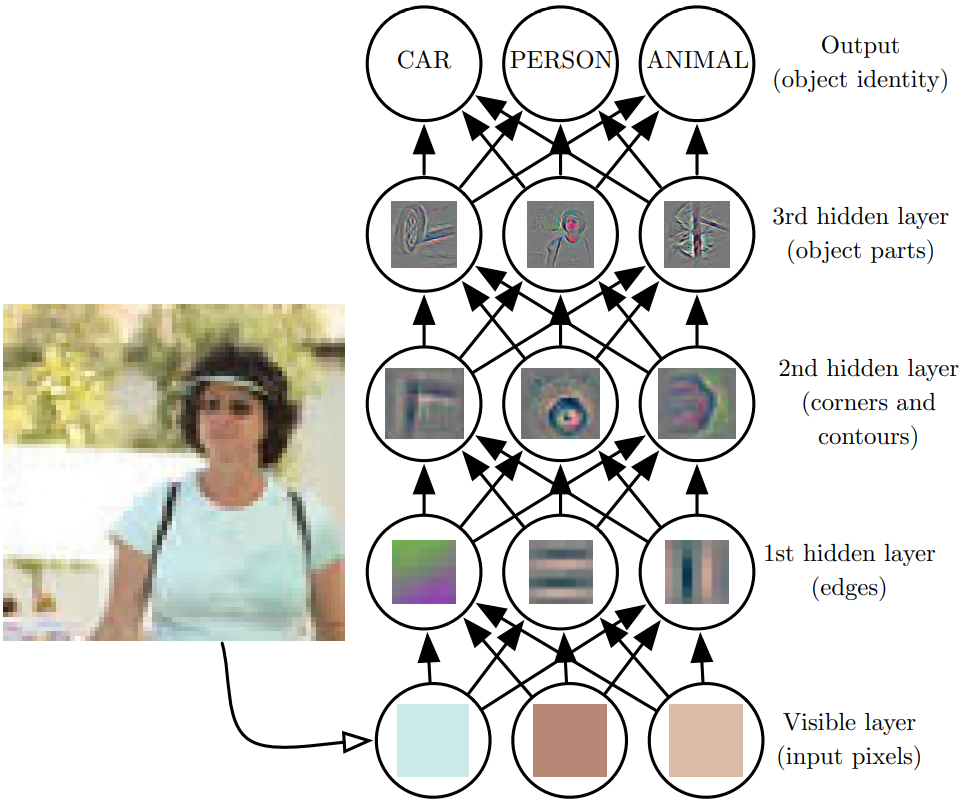
\includegraphics[scale=0.35]{Images/Chapter 6/ffdn-layers.png}
    \caption{Inner workings of a feedforward deep network}
    \source{Goodfellow et al. 2016}
    \label{fig:ch6-innerworkingsofaffdn}
\end{figure}

The idea of learning the right representation for the data provides one perspective on deep learning. A different one is that depth allows the computer to learn a multi-step computer program. Each layer of the representation can be thought of as the state of the computer’s memory after executing another set of instructions in parallel. Networks with greater depth can execute more instructions in sequence. Sequential instructions offer great power because later instructions can refer back to the results of previous ones.

The picture below sums up the differences between various types of artificial intelligence-based systems:

\begin{figure}[hbt]
    \centering
    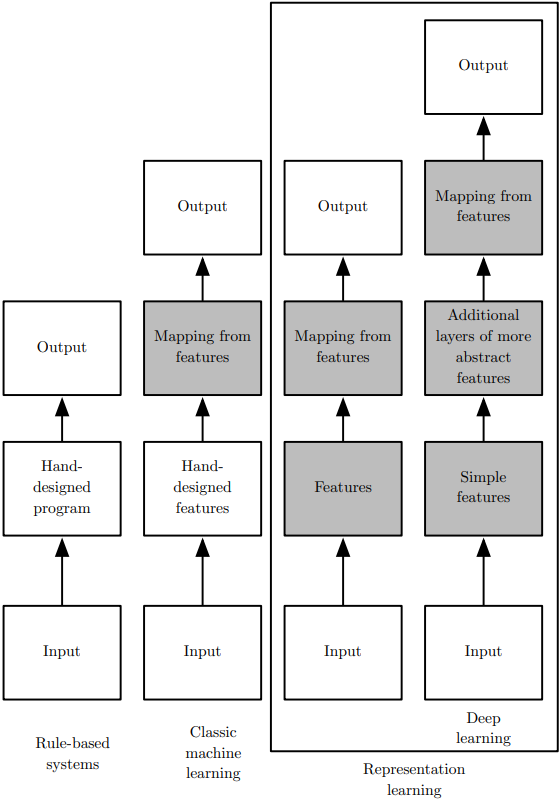
\includegraphics[scale=0.6]{Images/Chapter 6/types-ai.png}
    \caption{Differences between various types of AI-based systems}
    \source{Goodfellow et al. 2016}
    \label{fig:ch6-aitypesdifferences}
\end{figure}